\documentclass[11pt,]{article}
\usepackage{mathpazo}
\usepackage{amssymb,amsmath}
\usepackage{ifxetex,ifluatex}
\usepackage{fixltx2e} % provides \textsubscript
\ifnum 0\ifxetex 1\fi\ifluatex 1\fi=0 % if pdftex
  \usepackage[T1]{fontenc}
  \usepackage[utf8]{inputenc}
\else % if luatex or xelatex
  \ifxetex
    \usepackage{mathspec}
    \usepackage{xltxtra,xunicode}
  \else
    \usepackage{fontspec}
  \fi
  \defaultfontfeatures{Mapping=tex-text,Scale=MatchLowercase}
  \newcommand{\euro}{€}
\fi
% use upquote if available, for straight quotes in verbatim environments
\IfFileExists{upquote.sty}{\usepackage{upquote}}{}
% use microtype if available
\IfFileExists{microtype.sty}{%
\usepackage{microtype}
\UseMicrotypeSet[protrusion]{basicmath} % disable protrusion for tt fonts
}{}
\usepackage{natbib}
\bibliographystyle{amnat}
\usepackage{graphicx}
\makeatletter
\def\maxwidth{\ifdim\Gin@nat@width>\linewidth\linewidth\else\Gin@nat@width\fi}
\def\maxheight{\ifdim\Gin@nat@height>\textheight\textheight\else\Gin@nat@height\fi}
\makeatother
% Scale images if necessary, so that they will not overflow the page
% margins by default, and it is still possible to overwrite the defaults
% using explicit options in \includegraphics[width, height, ...]{}
\setkeys{Gin}{width=\maxwidth,height=\maxheight,keepaspectratio}
\ifxetex
  \usepackage[setpagesize=false, % page size defined by xetex
              unicode=false, % unicode breaks when used with xetex
              xetex]{hyperref}
\else
  \usepackage[unicode=true]{hyperref}
\fi
\hypersetup{breaklinks=true,
            bookmarks=true,
            pdfauthor={Matthew A. Barbour\^{}\{1,2,\textbackslash{}ast\}; Christopher J. Greyson-Gaito\^{}\{1,3\}; Arezoo Sootodeh\^{}\{3\}; Brendan Locke\^{}\{4\}; Jordi Bascompte\^{}\{2\}},
            pdftitle={Phenotypic evolution is more constrained in simpler food webs},
            colorlinks=true,
            citecolor=blue,
            urlcolor=black,
            linkcolor=black,
            pdfborder={0 0 0}}
\urlstyle{same}  % don't use monospace font for urls
\setlength{\parindent}{0pt}
\setlength{\parskip}{6pt plus 2pt minus 1pt}
\setlength{\emergencystretch}{3em}  % prevent overfull lines
\setcounter{secnumdepth}{0}

%%% Use protect on footnotes to avoid problems with footnotes in titles
\let\rmarkdownfootnote\footnote%
\def\footnote{\protect\rmarkdownfootnote}


  \title{Phenotypic evolution is more constrained in simpler food webs}
    \author{Matthew A. Barbour\(^{1,2,\ast}\) \\ Christopher J. Greyson-Gaito\(^{1,3}\) \\ Arezoo Sootodeh\(^{3}\) \\ Brendan Locke\(^{4}\) \\ Jordi Bascompte\(^{2}\)}
    \date{}
  
%%% From AmNat_MS_template.tex
%\documentclass[11pt]{article}
%\usepackage[sc]{mathpazo} %Like Palatino with extensive math support
\usepackage{fullpage}
%\usepackage[authoryear,sectionbib,sort]{natbib}
\linespread{1.7}
%\usepackage[utf8]{inputenc}
\usepackage{lineno}

%%%%%%% Sections not currently working properly
%\usepackage{titlesec}
%\titleformat{\section}[block]{\Large\bfseries\filcenter}{\thesection}{1em}{}
%\titleformat{\subsection}[block]{\Large\itshape\filcenter}{\thesubsection}{1em}{}
%\titleformat{\subsubsection}[block]{\large\itshape}{\thesubsubsection}{1em}{}
%\titleformat{\paragraph}[runin]{\itshape}{\theparagraph}{1em}{}[. ]\renewcommand{\refname}{Literature Cited}

%%% My added packages
%\usepackage{amsmath} % for matrices
%\usepackage{graphicx} % for organizing figures
%\usepackage{lmodern} % for tilde
%\usepackage[T1]{fontenc} % for tilde

%%%%%%%%% Previous - likely useful though
%\usepackage{setspace}\doublespacing
%\usepackage{float}
%\let\origfigure\figure
%\let\endorigfigure\endfigure
%\renewenvironment{figure}[1][2] {
%    \expandafter\origfigure\expandafter[H]
%} {
%    \endorigfigure
%}

\begin{document}

\maketitle


\noindent 1. University of British Columbia, Department of Zoology,
Vancouver, BC V6T 1Z4, Canada;

\noindent 2. University of Zurich, Department of Evolutionary Biology
and Environmental Studies, Winterthurerstrasse 190, 8057 Zurich,
Switzerland;

\noindent 3. University of Guelph, Department of Integrative Biology,
Guelph, ON N1G 2W1, Canada;

\noindent 4. Humboldt State University, Department of Biological
Sciences, Arcata, CA 95521, USA.

\(^\ast\) Corresponding author; e-mail:
\href{mailto:matthew.barbour@ieu.uzh.ch}{\nolinkurl{matthew.barbour@ieu.uzh.ch}}

\bigskip

\emph{Manuscript elements}: Figure 1, figure 2, figure 3, figure 4. All
figures should be printed in color.

\bigskip

\emph{Keywords}: fitness landscape, host-parasitoid, natural selection,
G-matrix, community context, ecological networks, evolutionary ecology,
eco-evolutionary dynamics.

\bigskip

\emph{Manuscript type}: Article.

\bigskip

\footnotesize Prepared using an \emph{Am. Nat.} inspired \LaTeX{}
template for Rmarkdown. \normalsize

\linenumbers{} \modulolinenumbers[3]

\newpage

\section{Abstract}\label{abstract}

Global change is simplifying the structure of ecological networks;
however, we are currently in a poor position to predict how these
simplified communities will affect the evolutionary potential of
remaining populations. Theory on adaptive landscapes provides a
framework for predicting how selection constrains phenotypic evolution,
but often treat the community context of evolving populations as a
``black box''. Here, we integrate ecological networks and adaptive
landscapes to examine how changes in food-web complexity shape
evolutionary constraints. We conducted a field experiment that
manipulated the diversity of insect parasitoids (food-web complexity)
that were able to impose selection on an insect herbivore. We then
measured herbivore survival as a function of three key phenotypic
traits. We found that more traits were under selection in simpler
vs.~more complex food webs. The adaptive landscape was more neutral in
complex food webs because different parasitoid species impose different
selection pressures, minimizing relative fitness differences among
phenotypes. Our results suggest that phenotypic evolution becomes more
constrained in simplified food webs. This indicates that the
simplification of ecological communities may constrain the adaptive
potential of remaining populations to future environmental change.

\newpage

\begin{quote}
``What escapes the eye, however, is a much more insidious kind of
extinction: the extinction of ecological interactions.''
\citet{Janzen1974}
\end{quote}

\section{Introduction}\label{introduction}

The adaptive landscape provides a powerful framework for understanding
how natural selection has shaped the evolution of biodiversity ---from
genes to phenotypes to species
\citep{Wright1931, Simpson1944, Arnold2001}. More than a metaphor, the
adaptive landscape links quantitative genetic and phenotypic variation
to evolution by natural selection
\citep{Lande1979, Arnold1984applications, Arnold1984theory}. Ecological
interactions often play a key role in shaping adaptive landscapes, as
evidenced by the role of antagonistic \citep{Schluter2000, Abrams2000}
and mutualistic \citep{Bronstein2006} interactions in driving
evolutionary change. Although there is clear evidence that pairwise
interactions can shape the adaptive landscape, we do not know how the
adaptive landscape is shaped by the community context
\citep{McPeek2017, terHorst2018}. Resolution on how the community
context shapes phenotypic evolution is urgently needed though, given the
rapid impacts of climate change on ecological communities
\citep{Scheffers2016}.

Ecological networks, such as food webs describing who-eats-whom in
ecological communities, provide an explicit representation of the
community context \citep{Bascompte2014, McCann2012}. Here, we integrate
ecological networks and adaptive landscapes to understand how community
context constrains evolutionary change \citep{Arnold1992}. Different
aspects of evolutionary constraints can be inferred by quantifying the
slope and curvature of the adaptive landscape. For example, the slope is
determined by directional selection gradients acting on each phenotypic
trait and influences the trajectory of evolutionary change
\citep{Lande1979, Arnold1992}. Evolutionary trajectories become more
constrained with an increase in the number of traits under selection, as
this diminishes the number of optimal solutions \citep{Arnold2003}. The
curvature of the adaptive landscape can also constrain evolution through
its indirect effect on genetic constraints
\citep{Arnold1992, Hansen2008}. Genetic constraints are largely governed
by a population's \textbf{G}-matrix ---the additive genetic variances
and covariances between traits \citep{Hansen2008}. In general, genetic
constraints will increase with the number of traits under directional or
stabilizing selection, as this will decrease the additive genetic
variance in those traits \citep{Hansen2008}. Genetic constraints may
also increase with the number of trait combinations under correlational
selection, as this type of selection decreases the evolutionary
independence of traits \citep{Hansen2008}. If we want to predict how
community context constrains evolutionary change, we must understand how
ecological networks shape the adaptive landscape.

Global change is simplifying the structure of ecological communities,
which may influence evolutionary constraints in a number of ways. For
example, in a multitrophic community or food web, if different consumers
impose directional selection on different traits of a shared resource,
then more complex food webs may constrain evolution by increasing the
number of traits under selection. Alternatively, if consumers impose
selection on different values of a trait, then their selective effects
would cancel each other out in more complex food webs. To examine these
different possibilities (among others), we conducted a field experiment
that manipulated the complexity of trophic interactions (hereafter
food-web complexity) associated with an abundant insect herbivore
(\emph{Iteomyia salicisverruca}; Family Cecidomyiidae)(fig.
\ref{fig:Conceptual}). The larvae of this herbivore induce tooth-shaped
galls when they feed on the developing leaves of willow trees
\citep[\emph{Salix} sp.,][]{Russo2006}. These galls protect larva from
attack by generalist predators (e.g.~ants, spiders), but they suffer
high mortality from egg and larval parasitoids \citep{Barbour2016}. We
manipulated food-web complexity by either excluding the guild of larval
parasitoids (simple food web) or allowing both egg and larval
parasitoids to impose selection on gall midge traits (complex food web;
fig. \ref{fig:Conceptual}). We then applied modern statistical methods
to quantify the effect of food-web complexity on the slope and curvature
of the gall midge's adaptive landscape. Taken together, our study gives
insight to how local extinctions, and concomitant decreases in food-web
complexity, may constrain the evolution of interacting populations.

\section{Methods}\label{methods}

\subsection{Study Site}\label{study-site}

We conducted our study within a four-year old common garden experiment
of coastal willow (\emph{Salix hookeriana}) located at Humboldt Bay
National Wildlife Refuge (HBNWR) (40 40'53``N, 124 12'4''W) near Loleta,
California, USA. This common garden consists of 26 different willow
genotypes that were collected from a single population of willows
growing around Humboldt Bay. Stem cuttings of each genotype (25
replicates per genotypes) were planted in a completely randomized design
in two hectares of a former cattle pasture at HBNWR. Willows at our
study site begin flowering in February and reach their peak growth in
early August. During this study, willows had reached 5 - 9m in height.
Further details on the genotyping and planting of the common garden are
available in \citet{Barbour2015}.

\subsection{Manipulating Food-web
Complexity}\label{manipulating-food-web-complexity}

We setup our food-web manipulation across 128 plants soon after galls
began developing on willows in early June of 2013. These 128 plants came
from eight different plant genotypes that spanned the range of trait
variation observed in this willow population \citep{Barbour2015}. For
the complex food-web treatment (eight replicates per genotype), we used
flagging tape to mark 14 galled leaves per plant (\textasciitilde{}30
larvae), allowing the full suite of egg and larval parasitoids to impose
selection. Marking galls with flagging tape ensured that we compared
control and treatment galls with similar phenology when we collected
galls later in the season. For the simple food-web treatment, we
enclosed 14 galled leaves with 10x15cm organza bags (ULINE, Pleasant
Prairie, WI, USA) to exclude three parasitoid species that attack during
larval development. This treatment did not exclude the egg parasitoid
\emph{Platygaster} sp., which attacks prior to gall initiation
\citep[larva initiate gall development in Cecidomyiid
midges:][]{Gagne1989}. In late August, we collected marked and bagged
galls from each plant, placed them into 30 mL vials and kept them in the
lab for 4 months at room temperature. We then opened galls under a
dissecting scope and determined whether larvae survived to pupation (our
measure of fitness) or were parasitized. Since we were interested in
selection imposed by parasitoids, we excluded unknown sources of
mortality. For the food-web treatment that excluded larval parasitoids
(simple food web), we further restricted our data by removing any
incidental instances of parasitism by a larval parasitoid. This
represented less than 3\% of the observations in this food-web treatment
and allowed us to focus our inferences of selection on those imposed by
the egg parasitoid. Our final dataset contains survival estimates for
1285 larvae from 613 galls and 111 plants.

\subsection{Measuring Phenotypic
Traits}\label{measuring-phenotypic-traits}

We collected data on three different traits that we expected to
influence larval survival based on our previous work \citep{Barbour2016}
and others work with gall midges \citep{Weis1983, Heath2018}. First, we
measured gall diameter as the size of each gall chamber to the nearest
0.01 mm at its maximum diameter (perpendicular to the direction of plant
tissue growth). Our previous work has shown that larger galls are
associated with higher survival \citep{Barbour2016}. Second, we measured
clutch size by counting the number of chambers in each gall
\citep{Weis1983, Heath2018}. All larvae collected from the same
multi-chambered gall were scored with the same clutch size. Third, we
measured oviposition preference as the density of larvae observed on a
plant in an independent survey. We did this by randomly sampling five
branches per tree and counting the number of individual gall chambers
(number of larvae). We then converted these counts to a measure of
larval density per 100 shoots by counting the number of shoots on the
last branch we sampled. All larvae collected from the same plant were
scored with the same oviposition preference. Measuring larval densities
on plants in the field is a common method for measuring oviposition
preference \citep{Gripenberg2010}; however, caution must be taken in
inferring `preference' as larval densities can be influenced by
processes other than preference \citep{Singer1986}. Fortunately, a
couple of features of our study system suggest that larval densities may
be a good proxy for oviposition preference. For example, since our data
comes from a randomized placement of plant genotypes in a common garden,
there is no consistent bias in which plant genotypes females are exposed
to while searching for oviposition sites. Also, egg predation is a minor
source of mortality for galling insects in general \citep{Hawkins1997};
therefore, we do not expect any prior egg predation to bias our
estimates of observed larval densities.

\subsection{Quantifying the Adaptive
Landscape}\label{quantifying-the-adaptive-landscape}

Our analyses consisted of three parts. First, we used generalized linear
mixed models (GLMM) to quantify selection surfaces \textemdash linear
and nonlinear relationships between absolute fitness (\(W\)) and
phenotypic traits (\(z_i\)) of individuals \textemdash in each food-web
treatment. Second, we translated selection surfaces into the scale of
relative fitness (\(w\)) in order to calculate selection gradients.
Third, we used our estimates of selection gradients to characterize the
slope and curvature of the adaptive landscape. Note that inferring
adaptive landscapes from selection surfaces assumes that trait
distributions are multivariate normal \citep{Lande1983}. To approximate
this assumption, we log-transformed clutch size and square-root
transformed oviposition preference. We then scaled all phenotypic traits
(mean=0 and SD=1) in order to calculate standardized selection gradients
that were comparable across traits and with other studies of natural
selection.

\textbf{Selection surface}: Since larval survival was our measure of
absolute fitness, we used a GLMM that assumed a binomial error
distribution (and logit-link function). To approximate the selection
surface, we modelled larval survival as a function of food-web treatment
as well as linear (\(\alpha_{z_i}\)), quadratic (\(\alpha_{z_i:z_i}\)),
and linear interactions (\(\alpha_{z_i:z_j}\)) between each trait. We
also allowed these trait-fitness relationships (\(\alpha\)) to vary
between food-web treatments. Note that to obtain valid estimates of
linear trait-fitness relationships, we removed nonlinear terms prior to
estimating linear relationships \citep{Lande1983}. Other approaches have
been advocated for approximating selection surfaces
\citep{Schluter1988}; however, our approach enables us to calculate
selection gradients, and thus is more appropriate for approximating the
adaptive landscape \citep{Arnold2003}. To account for the
nonindependence of clutch size (measured at gall level) and oviposition
preference (measured at plant level) as well as any independent effects
of willow genotype on larval survival, we modelled gall ID nested within
plant ID nested within genotype ID as random effects. Although
statistical models with random effects are not common in analyses of
natural selection, we think that modelling random effects can mitigate
biased estimates of selection due to environmental covariances between
traits and fitness \citep{Rausher1992}. Since our end goal was to
characterize the relationship between mean trait values and mean fitness
(adaptive landscape), we assumed the mean value of our random effects
(i.e., setting them to zero) when calculating trait-fitness
relationships. We then used parametric bootstrapping (1,000 replicates)
to estimate the effect of food-web treatment on larval survival as well
as trait-fitness relationships in each food-web treatment. To determine
whether trait-fitness relationships differed between food-web
treatments, we calculated the difference in bootstrapped replicates
between treatments.

\textbf{Selection gradients}: We used the method of \citet{Janzen1998}
to translate trait-fitness relationships (\(\alpha\)) into the scale of
relative fitness in order to calculate directional (\(\beta_{z_i}\)),
quadratic (\(\gamma_{z_i:z_i}\)), and correlational
(\(\gamma_{z_i:z_j}\)) selection gradients. Briefly, this method
calculates the average gradient of selection surfaces by multiplying the
average of \(W(z)[1-W(z)]\) by each regression coefficient (e.g.
\(\alpha_{z_i}\), \(\alpha_{z_i:z_i}\), or \(\alpha_{z_i:z_j}\)). We
then divided this average gradient by mean fitness (\(\bar W\)) to put
it on the scale of relative fitness, and thus interpretable as a
selection gradient. We estimated selection gradients separately for each
food-web treatment. Note that we doubled all quadratic terms prior to
calculating selection gradients to put them on the same scale as
estimates of directional and correlational selection
\citep{Stinchcombe2008}.

\textbf{Evolutionary constraints}: We quantified the effects of food-web
complexity on evolutionary constraints by inspecting the slope and
curvature of the adaptive landscape. The number of selective constraints
is determined by the slope of the adaptive landscape, which in our study
corresponds to:

\[\text{Slope} = \beta = \begin{pmatrix} \beta_{\text{Diam}} \\ \beta_{\text{Clutch}} \\ \beta_{\text{Pref}} \end{pmatrix} \]
By comparing the number of traits that determine the slope (i.e.,
nonzero directional selection gradients) in simpler vs.~more complex
food webs, we can infer the effect of food-web complexity on selective
constraints.

The indirect effects of selection on genetic constraints is governed by
the curvature of the adaptive landscape
(\(\text{C}=\gamma - \beta \beta^\text{T}\)), which in our study
corresponds to:

\[\textbf{C} = \begin{pmatrix} \gamma_{\text{Diam:Diam}}&& \\ \gamma_{\text{Clutch:Diam}}&\gamma_{\text{Clutch:Clutch}}& \\ \gamma_{\text{Pref:Diam}} & \gamma_{\text{Pref:Clutch}} &\gamma_{\text{Pref:Pref}} \end{pmatrix} - \begin{pmatrix} \beta_{\text{Diam}}\beta_{\text{Diam}}&& \\ \beta_{\text{Clutch}}\beta_{\text{Diam}}&\beta_{\text{Clutch}}\beta_{\text{Clutch}}& \\ \beta_{\text{Pref}}\beta_{\text{Diam}} & \beta_{\text{Pref}}\beta_{\text{Clutch}} &\beta_{\text{Pref}}\beta_{\text{Pref}} \end{pmatrix}\]
\[\textbf{C} = \begin{pmatrix} C_{\text{Diam:Diam}}&& \\ C_{\text{Clutch:Diam}} & C_{\text{Clutch:Clutch}} & \\ C_{\text{Pref:Diam}} & C_{\text{Pref:Clutch}} & C_{\text{Pref:Pref}} \end{pmatrix}\]

Note that we ommitted the upper triangle of each matrix for clarity
since it is simply the reflection of the lower triangle. The sign of
diagonal terms of the curvature matrix dictate whether selection will
increase (+), decrease (-), or cause no change (0) in the additive
genetic variance of a trait. Similarly, any nonzero covariance terms
(off-diagonal) are indicative of selection for trait integration (i.e.,
less independence). Therefore, we can infer the indirect effects of
selection on genetic constraints by counting the number of negative
signs along the diagonal (decrease in additive genetic variance) and the
number of nonzero terms along the off-diagonal (trait integration) of
the curvature matrix.

\subsection{Adjusting for biased measurements of
selection}\label{adjusting-for-biased-measurements-of-selection}

Rather than imposing selection, parasitoids may influence the expression
of herbivore traits which could bias measurements of selection. In our
system, it was plausible that parasitoids may influence chamber diameter
by altering larval feeding behavior or killing larvae before they
complete their development. To estimate this potential bias, we subset
our data to only include galls where there was variation in larval
survival within the same gall (i.e.~1 \textgreater{} mean survival
\textgreater{} 0). If we assume that larvae within each gall should have
similar chamber diameters because they come from the same clutch and
experience the same local environment (an assumption our data supports:
gall ID explains 54\% of the variance in chamber diameter), then the
relationship between chamber diameter and larval survival in this data
subset represents the effect of parasitism on trait expression
(i.e.~bias). We used a GLMM with the same structure as described above
except that we only modelled a linear relationship between chamber
diameter and larval survival (\(\alpha_{\text{Diam}}\)). We detected a
positive bias in both food-web treatments (complex
\(\alpha_{\text{Diam}}\)= 0.36 {[}0.05, 0.67{]}; simple
\(\alpha_{\text{Diam}}\)= 0.42 {[}0.01, 0.82{]}), indicating that
unadjusted relationships would overestimate the strength of selection on
chamber diameter. To account for this bias, we substracted our mean
estimates of bias from our estimates with the full dataset prior to
calculating chamber diameter's trait-fitness relationship and
directional selection gradient.

\subsection{Measuring selection on the extended phenotype of egg
parasitoids}\label{measuring-selection-on-the-extended-phenotype-of-egg-parasitoids}

Once parasitized, the gall phenotype becomes the extended phenotype of
the egg parasitoid. This extended phenotype may influence the egg
parasitoid's survival in the face of larval parasitoids, and thus
experiences selection. Our food-web manipulation allows us to measure
selection imposed by larval parasitoids on the extended phenotype of egg
parasitoids. Using the same models as described above, we substituted
egg parasitism as our response variable to quantify trait-fitness
relationships and selection gradients acting on the egg parasitoid. Note
that we cannot test the effect of food-web complexity on the egg
parasitoid's adaptive landscape ---we can only estimate the selection
imposed by larval parasitoids. This comparison is still useful though in
determining the extent to which the community context may have indirect
evolutionary effects by altering selection on multiple interacting
populations.

All analyses and visualizations were conducted in R \citep{R2018}.
Unless otherwise noted, we report mean estimates of trait-fitness
relationships and selection gradients with 95\% confidence intervals in
brackets. Note that for visualizing the adaptive landscape we restrict
trait axes to \(\pm 1\) SD of the mean trait value. This emphasizes the
fact that we can only reliably estimate the shape of the adaptive
landscape near the mean phenotype of the population \citep{Arnold2001}.
We also plot mean larval survival on a natural log scale to accurately
reflect the mathematical definition of the adaptive landscape
\citep{Arnold2003}.

\section{Results}\label{results}

\subsection{Simpler food webs increase selective
constraints}\label{simpler-food-webs-increase-selective-constraints}

\indent We found that more gall midge traits experienced directional
selection in the simple (3 of 3) vs.~complex food-web treatment (1 of
3)(table \ref{Table:Gradients}). For example, we observed directional
selection for smaller clutch sizes in the simple food web, but there was
no evidence of selection acting on this trait in the complex food web
(table \ref{Table:Gradients}; fig. \ref{fig:UV_Landscape}C). This
absence of selection appeared to be a result of conflicting selection
pressures imposed by each guild of parasitoids (fig.
\ref{fig:UV_Landscape}). Specifically, when we subset our data to focus
on differences between parasitoid guilds, we found that larval
parasitoids actually impose directional selection for larger clutch
sizes (\(\beta_{\text{Clutch}}\)= 0.13 {[}0.03, 0.23{]}). In the simple
food web, we also observed clear evidence of directional selection for
midges to avoid ovipositing on plants with high densities of
conspecifics (table \ref{Table:Gradients}; fig.
\ref{fig:UV_Landscape}B); however, this relationship was weaker in
complex food webs (table \ref{Table:Gradients}). This was likely a
result of larval parasitoids imposing greater mortality on egg
parasitoids at high gall midge densities (see Selection on the extended
phenotype of egg parasitoids section), and thus a less than additive
effect on gall midges. Chamber diameter experienced positive directional
selection in both food-web treatments, but selection was 65\% higher in
complex food webs (table \ref{Table:Gradients}; fig.
\ref{fig:UV_Landscape}). This was not due to any difference between egg
and larval parasitoids (fig. \ref{fig:UV_Landscape}), but was due to the
lower average survival in complex food webs (contrast -0.26 {[}-0.12,
-0.42{]}).

\subsection{Simpler food webs increase genetic
constraints}\label{simpler-food-webs-increase-genetic-constraints}

\indent The curvature of the adaptive landscape indirectly affects
genetic constraints and is influenced by directional, quadratic, and
correlational selection gradients. Our food-web treatment did not alter
correlational selection for any combination of traits (table
\ref{Table:Gradients}). Similarly, our food-web treatment did not
influence quadratic selection on either chamber diameter or clutch size
(table \ref{Table:Gradients}; fig. \ref{fig:UV_Landscape}A,C). In
contrast, our food-web treatment did alter quadratic selection acting on
oviposition preference (table \ref{Table:Gradients}). The negative
relationship between oviposition preference and larval survival dampened
at high densities in complex, but not simple food webs (fig.
\ref{fig:UV_Landscape}B). This dampened relationship was partly due to a
trend for nonlinear selection imposed by larval parasitoids
(\(\gamma_{\text{Pref:Pref}}\)= 0.18 {[}-0.01, 0.42{]}), but was also
magnified by the lower average survival in complex food webs.

To estimate the net effect of food-web complexity on the curvature
(\(C\)) of the adaptive landscape, we only retained nonzero selection
gradients (i.e.~95\% CI did not overlap zero) prior to calculating the
curvature (\(\gamma - \beta \beta^\text{T}\)) in each food-web
treatment. We found that the curvatures of the adaptive landscape
exhibited the following structures:

\[\textbf{C} = \begin{pmatrix} C_{\text{Diam:Diam}}&& \\ C_{\text{Clutch:Diam}} & C_{\text{Clutch:Clutch}} & \\ C_{\text{Pref:Diam}} & C_{\text{Pref:Clutch}} & C_{\text{Pref:Pref}} \end{pmatrix}\]

\[\textbf{C}_{\text{Complex}} = \begin{pmatrix} 
-0.12 &  &  \\  
0 & 0 &  \\  
0 & 0 & 0.33 \end{pmatrix}\]

\[\textbf{C}_{\text{Simple}} = \begin{pmatrix} 
-0.04 &  &  \\  
0.02 & -0.01 &  \\  
0.03 & -0.01 & -0.03 \end{pmatrix}\]

Remember that we can infer the indirect effects of selection on genetic
constraints by counting the number of negative signs along the diagonal
(decrease in additive genetic variance) and the number of nonzero terms
along the off-diagonal (trait integration) of the curvature matrix. The
structure of these matrices indicates that there are more selective
constraints imposed on the gall midge in the simpler (6 of 6) vs.~more
complex (1 of 6) food web. Simpler food webs acted to decrease genetic
variance for all three phenotypic traits (negative diagonal terms),
whereas only one trait (chamber diameter) experienced a decrease in
additive genetic variance in the more complex food web. For genetic
covariances, the simpler food web favored integration among all three
phenotypic traits (nonzero off-diagonal terms), and thus constraints
along all three axes of covariance (fig. \ref{fig:MV_Landscape}). In
contrast, there was no strong evidence of trait integration in the more
complex food web (fig. \ref{fig:MV_Landscape}).

\subsection{Selection on the extended phenotype of egg
parasitoids}\label{selection-on-the-extended-phenotype-of-egg-parasitoids}

Gall midge preference influenced the probability of observing egg
parasitoids in complex vs.~simple food webs (contrast
\(\alpha_{\text{Pref}}\)= 1 {[}0.03, 2.22{]} ). Specifically, larval
parasitoids decreased the probability of observing egg parasitoids at
high gall midge densities (fig. \ref{fig:EggPtoid_Selection}). Note
however that this trait-fitness relationship did not translate into a
significant difference in selection (contrast \(\beta_{\text{Pref}}\)=
0.24 {[}-0.09, 0.62{]} ). This was likely because there was a tendency
(albeit not statistically signficant) for a lower probability of
egg-parasitoid survival in complex vs.~simple food webs (contrast=0.1
{[} -0.08, 0.31{]}), which masks this trait-fitness relationship. We
also observed two other interesting trends, although neither
significantly differed between treatments. Specifically, there was a
tendency for the impact of larval parasitoids to increase nonlinearly at
higher gall midge densities (fig. \ref{fig:EggPtoid_Selection}; complex
\(\alpha_{\text{Pref:Pref}}\)= -0.49 {[}-1.08, -0.1{]}; but contrast
\(\alpha_{\text{Pref:Pref}}\)= 0.46 {[}-0.03, 1.1{]}). There was also a
tendency for egg parasitoids to obtain a refuge in large gall chambers
at high gall midge densities (complex \(\alpha_{\text{Pref:Diam}}\)=
0.25 {[}0.02, 0.5{]}; but contrast \(\alpha_{\text{Pref:Diam}}\)= -0.25
{[}-0.57, 0.04{]}).

\section{Discussion}\label{discussion}

Our key finding was that phenotypic evolution in gall midges was more
constrained in simpler food webs. More traits contributed to the slope
of the adaptive landscape in the simpler food web, suggesting that the
trajectory of phenotypic evolution is more constrained. Similarly, the
simple food-web treatment indirectly increased the number of genetic
constraints, which could act to constrain the gall midge's adaptive
potential in the face of novel selection pressures. We also found
evidence of indirect selection pressures in more complex food webs,
suggesting that the adaptive landscape may be more dynamic in complex
food webs. Taken together, our study provides experimental evidence from
the field that the simplification of ecological communities may
constrain the adaptive potential of remaining populations.

All three phenotypic traits we examined experienced directional
selection in the simpler food web, indicating that there is an optimal
phenotype that maximizes larval survival (i.e.~large chamber diameter,
small clutch size, and avoidance of conspecifics). In contrast, we did
not observe selective constraints on clutch size and oviposition
preference in the more complex food web. This suggests that there are
many optimal phenotypes (adaptive peaks), or in this case, a flat
adaptive landscape where there are no fitness consequences for
phenotypic change in these traits. This also implies that as selective
constraints dampen in more complex food webs, then the trajectory of
evolution becomes more determined by genetic constraints. This is made
clear if we inspect the `Lande equation', \(\Delta z = \text{G} \beta\),
where G corresponds to the population's G-matrix. As the components of
\(\beta\) go to zero, then \(\Delta z\) is more influenced by the
G-matrix. Interestingly, this corresponds to \citet{Schluter1996}`s
hypothesis that phenotypic evolution often follows 'genetic lines of
least resistance'. \citet{Schluter1996} found support for this
hypothesis from data on natural populations of several vertebrate
species, including threespine sticklebacks, a few species of songbirds,
and mice from the genus \emph{Peromyscus}. All of these species occupy
intermediate trophic levels and are likely embedded in complex food
webs, which is consistent with our suggestion that genetic constraints
may have a stronger influence in more complex food webs.

We also found evidence for more genetic constraints in simpler food webs
due to indirect effects of selection on the population's G-matrix. The
ability of a population to adapt to novel selection pressures
(evolvability) is largely governed by the structure of its G-matrix
\citep{Hansen2008}. When selection favors genetic covariance between
traits (positive or negative), this results in less autonomy of
evolutionary responses to changing environments. Similarly, decreases in
genetic variance constrain potential for the trait itself to evolve.
Together, this suggests that simpler food webs may decrease the
evolutionary potential of populations by indirectly selecting for
decreases in genetic variance in multiple traits and favoring trait
integration. Current theory often assumes genetic variances and
covariances remain constant over time rather than dynamically changing
with the community context \citep{McPeek2017, Guimaraes2017}. Our
empirical results highlight the need to explore the evolutionary
consequences of not only direct effects of selection, but indirect
effects on genetic constraints that are shaped by the community context.

The generality of our results likely depends on the relative abundance
and functional differences between consumers in a community. In the
simplest case, when consumers do not differ from each other, then we do
not expect changes in food-web complexity to modify selective
constraints. Also, many consumers may be at too low of abundances to
impose selection on their resources. Rank abundance curves
\citep{Preston1948} and the disproportionate number of weak interactions
in diverse communities \citep{Paine1992} support this notion. When
consumers are abundant though, the effect of food-web complexity will
depend on whether different species impose conflicting selection
pressures or select for distinct traits. For example, parisitoids and
birds impose conflicting selection pressures on the size of galls
induced by the fly \emph{Eurosta solidaginis}
\citep{Weis1985, Abrahamson1997, Start2016}. Recent studies in this
system have shown that decreases in the relative abundance of birds, due
to either small patch sizes \citep{Start2016} or proximity to urban
areas \citep{Start2018} causes a shift from neutral to directional
selection on gall size. On the other hand, different consumers may
impose selection on different traits, favoring trait integration and
increasing genetic constraints. Examples of this include strong genetic
covariances in plant resistance to different insect herbivores
\citep{Maddox1990, Wise2007, Wise2013}, although there are also examples
where these covariances are weak \citep{Roche1997, Barbour2015}, or vary
from year-to-year \citep{Johnson2007}. We suggest that gaining
predictive insight to the effects of food-web disassembly requires an
understanding of the mechanisms governing the assembly of trophic
interactions.

Our results suggest that the simplification of ecological communities
may not only directly affect connected species, but also result in
indirect evolutionary effects. In our study, this indirect effect arises
from egg parasitoids being released from intraguild predation in simpler
food webs. This release occurs more on trees with high larval densities,
which could intensify selection on gall midge oviposition preference. A
growing number of experiments over the past two decades have
demonstrated the presence and potential importance of indirect
evolutionary effects that emerge in a community context
\citep{Juenger1998, Stinchcombe2001, Lankau2007, Walsh2008, Walsh2010, terHorst2010, Sahli2011, Lau2012, terHorst2015, Schiestl2018}.
If indirect evolutionary effects are common \citep{Walsh2013}, then
predicting evolutionary trajectories resulting from the simplification
of food webs will require evolutionary studies to explicitly account for
the ecological networks that species are embedded in.

There are a growing number of theoretical studies on adaptation to
directional environmental change that incorporate species interactions
\citep[e.g.][]{deMazancourt2008, Johansson2008, Norberg2012, Osmond2017PredatorsHelpPrey}.
This work has given insight to the mechanisms by which pairwise
interactions modify the adaptive potential of species. Our study hints
at a novel mechanism, whereby food-web complexity flattens the adaptive
landscape, thus facilitating future adaptation by allowing genetic and
phenotypic variation to persist. This mechanism only emerges once we
move beyond pairwise interactions to consider selection on multiple
traits in a community context. However, a study on competition has
highlighted that we may expect the opposite effect of species diversity
in competitive communities \citep{deMazancourt2008}. This negative
effect of species diversity on adaptation occurs because there is a
greater chance that the optimal phenotype is already occupied by a
competitor in a more diverse community. More work is needed to examine
how the distribution of different interaction types affects adaptation
to environmental change in species-rich communities.

Our study gives insight to how local extinctions, and concomitant
decreases in food-web complexity, increase evolutionary constraints.
This hints at a potential insidious effect of local extinctions that
compromises the robustness of remaining populations to future
environmental change. Our work also highlights some key challenges for
predicting phenotypic evolution in the face of global change. First, the
simplification of ecological communities may actually reduce the
predictability of phenotypic evolution, because knowledge is required of
both selective and genetic constraints, rather than potentially just
genetic constraints in more complex systems. Second, many theoretical
models of eco-evolutionary dynamics focus on phenotypic change in a
single trait, yet our results highlight that the number of traits under
selection may change with the community context. Importantly, while the
net effects of selection in complex communities may be dampened, we
still found that different species/guilds imposed different selection
pressures. Knowing these hidden selection pressures is critical for
prediction, because the trajectory of evolution will depend on the
nature of change in the community context. We expect that a continued
integration of adaptive landscapes and ecological networks will enhance
our ability to predict the evolutionary consequences of changes in
ecological communities.

\section{Acknowledgements}\label{acknowledgements}

We thank the staff of Humboldt Bay National Wildlife Refuge (U.S. Fish
and Wildlife Service) for facilitating experimental logistics. For
assistance with fieldwork, we thank Ruthie Espanol and Andrew MacDonald.
For funding support, we thank the University of British Columbia (James
Robert Thompson Fellowship and Four-Year Fellowship to M.A.~Barbour),
NSERC (Discovery grant to Greg Crutsinger), and the Swiss National
Science Foundation (grant 31003A\_160671 to J. Bascompte).

\section{References}\label{references}

\hypertarget{refs}{}

\newpage 

\section{Tables}\label{tables}

\begin{table}[h]
\caption{Standardized selection gradients acting on gall midges in complex vs. simple food webs.}
\label{Table:Gradients}
\centering
\begin{tabular}{lccc}
\\ 
\hline
\textbf{Selection gradient} & \textbf{Complex} & \textbf{Simple} & \textbf{Contrast}  \\ 
\hline
$\beta_{\text{Diam}}$ & 
\textbf{
0.34 [
0.22,
0.47] }& 
\textbf{
0.21 [
0.13,
0.3] }& 

-0.13 [
-0.26,
0.01] \\

$\beta_{\text{Clutch}}$ & 
0.06 [
-0.04,
0.17] & 
\textbf{
-0.09 [
-0.18,
-0.02] }& 
\textbf{
-0.15 [
-0.29,
-0.02] }\\

$\beta_{\text{Pref}}$ &
-0.12 [
-0.29,
0.05] & 
\textbf{
-0.16 [
-0.25,
-0.07] }& 

-0.04 [
-0.22,
0.14] \\

$\gamma_{\text{Diam,Diam}}$ &
0.14 [
-0.06,
0.32] & 

0.1 [
-0.03,
0.25] & 

-0.04 [
-0.27,
0.2] \\

$\gamma_{\text{Clutch,Clutch}}$ & 
-0.05 [
-0.25,
0.16] & 

-0.12 [
-0.27,
0.03] & 

-0.06 [
-0.33,
0.19] \\

$\gamma_{\text{Pref,Pref}}$ & 
\textbf{
0.33 [
0.06,
0.64] }& 

0.01 [
-0.14,
0.17] & 
\textbf{
-0.32 [
-0.66,
0] }\\

$\gamma_{\text{Diam,Clutch}}$ & 
-0.05 [
-0.17,
0.08] & 

-0.07 [
-0.15,
0.02] & 

-0.02 [
-0.16,
0.13] \\

$\gamma_{\text{Diam,Pref}}$ & 
-0.13 [
-0.28,
0] & 

-0.02 [
-0.09,
0.06] & 

0.12 [
-0.05,
0.29] \\

$\gamma_{\text{Clutch,Pref}}$ & 
0.03 [
-0.11,
0.18] & 

0 [
-0.07,
0.07] & 

-0.03 [
-0.19,
0.12] \\ 
\hline
\end{tabular}
\bigskip{}
\\
{\footnotesize Note: Values in brackets represent 95\% confidence intervals. Bold values indicate that the 95\% CI does not overlap zero. $\beta_{\text{Diam}}$ has been adjusted for bias.}
\end{table}

\newpage 

\begin{table}[h]
\caption{Relationship between absolute fitness (larval survival) and phenotypic traits of gall midges in complex vs. simple food webs.}
\label{Table:Coefs}
\centering
\begin{tabular}{lccc}
\\ 
\hline
\textbf{Coefficient} & \textbf{Complex} & \textbf{Simple} & \textbf{Contrast}  \\ 
\hline
$\alpha_{\text{Diam}}$ & 
\textbf{
1.14 [
0.73,
1.57] }& 
\textbf{
1.1 [
0.68,
1.58] }& 

-0.04 [
-0.57,
0.51] \\

$\alpha_{\text{Clutch}}$ & 
0.21 [
-0.13,
0.57] & 
\textbf{
-0.47 [
-0.94,
-0.09] }& 
\textbf{
-0.68 [
-1.27,
-0.13] }\\

$\alpha_{\text{Pref}}$ &
-0.41 [
-0.97,
0.15] & 
\textbf{
-0.84 [
-1.35,
-0.36] }& 

-0.43 [
-1.16,
0.25] \\

$\alpha_{\text{Diam,Diam}}$ &
0.23 [
-0.1,
0.54] & 

0.27 [
-0.07,
0.65] & 

0.04 [
-0.43,
0.52] \\

$\alpha_{\text{Clutch,Clutch}}$ & 
-0.09 [
-0.42,
0.26] & 

-0.31 [
-0.71,
0.08] & 

-0.22 [
-0.77,
0.31] \\

$\alpha_{\text{Pref,Pref}}$ & 
\textbf{
0.56 [
0.1,
1.07] }& 

0.03 [
-0.38,
0.46] & 

-0.52 [
-1.18,
0.09] \\

$\alpha_{\text{Diam,Clutch}}$ & 
-0.16 [
-0.57,
0.25] & 

-0.35 [
-0.78,
0.08] & 

-0.19 [
-0.78,
0.44] \\

$\alpha_{\text{Diam,Pref}}$ & 
-0.44 [
-0.95,
0.01] & 

-0.09 [
-0.5,
0.3] & 

0.36 [
-0.27,
0.97] \\

$\alpha_{\text{Clutch,Pref}}$ & 
0.1 [
-0.37,
0.59] & 

0 [
-0.37,
0.38] & 

-0.1 [
-0.69,
0.49] \\ 
\hline
\end{tabular}
\bigskip{}
\\
{\footnotesize Note: Values in brackets represent 95\% confidence intervals. Bold values indicate that the 95\% CI does not overlap zero. $\alpha_{\text{Diam}}$ has been adjusted for bias.}
\end{table}

\newpage 

\begin{figure}
\centering
\includegraphics{analyses/complex_simple_foodwebs_v2.jpeg}
\caption{\label{fig:Conceptual}Experimental manipulation of food-web
complexity associated with a leaf-galling midge (\emph{Iteomyia
salicisverruca}) feeding on the willow \emph{Salix hookeriana}. Black
arrows denote the flow of energy in this network of trophic
interactions. In the complex food-web treatment, we allowed the full
suite of egg and larval parasitoids to impose selection. In the simple
food-web treatment, we used mesh bags to exclude the guild of larval
parasitoids, only allowing the egg parasitoid (\emph{Platygaster} sp.)
to impose selection. Larval parasitoids include the following species
(from left to right): \emph{Mesopolobus} sp. (Family: Pteromalidae);
\emph{Tetrastichus} sp. (Family: Eulophidae); and \emph{Torymus} sp.
(Family: Torymidae).}
\end{figure}

\begin{figure}
\centering
\includegraphics{analyses/UV_landscapes.pdf}
\caption{\label{fig:UV_Landscape}Adaptive landscape of gall midge
phenotypes in complex vs.~simple food webs. Each panel corresponds to a
different phenotypic trait: chamber diameter (A); oviposition preference
(B); and clutch size (C). Solid lines represent selection experienced in
complex (orange) and simple (blue) food webs. Transparent lines
represent bootstrapped replicates to show the uncertainty in selection.
For clarity, we only display 100 bootstraps even though inferences are
based on 1,000 replicates. Note that mean larval survival is plotted on
a natural log scale to reflect the mathematical defintion of the
adaptive landscape.}
\end{figure}

\begin{figure}
\centering
\includegraphics{analyses/MV_landscapes.pdf}
\caption{\label{fig:MV_Landscape}Two dimensional view of adaptive
landscapes of gall midge phenotypes in complex vs.~simple food webs.
Each panel corresponds to a different combination of phenotypic traits:
clutch size and chamber diameter (A); clutch size and oviposition
preference (B); oviposition preference and chamber diameter (C). Arrows
represent mean estimates of directional selection gradients, while
contours represent predicted larval survival of the mean phenotype
(i.e., all traits = 0) in each food-web treatment. Notice that arrows
point more toward a corner of the adaptive landscape for each
combination of traits in the simple vs.~complex food-web treatment. This
indicates that trait integration (covariance) is more strongly favored
in simpler vs.~more complex food webs. Note that mean larval survival is
plotted on a natural log scale to reflect the mathematical definition of
the adaptive landscape.}
\end{figure}

\begin{figure}
\centering
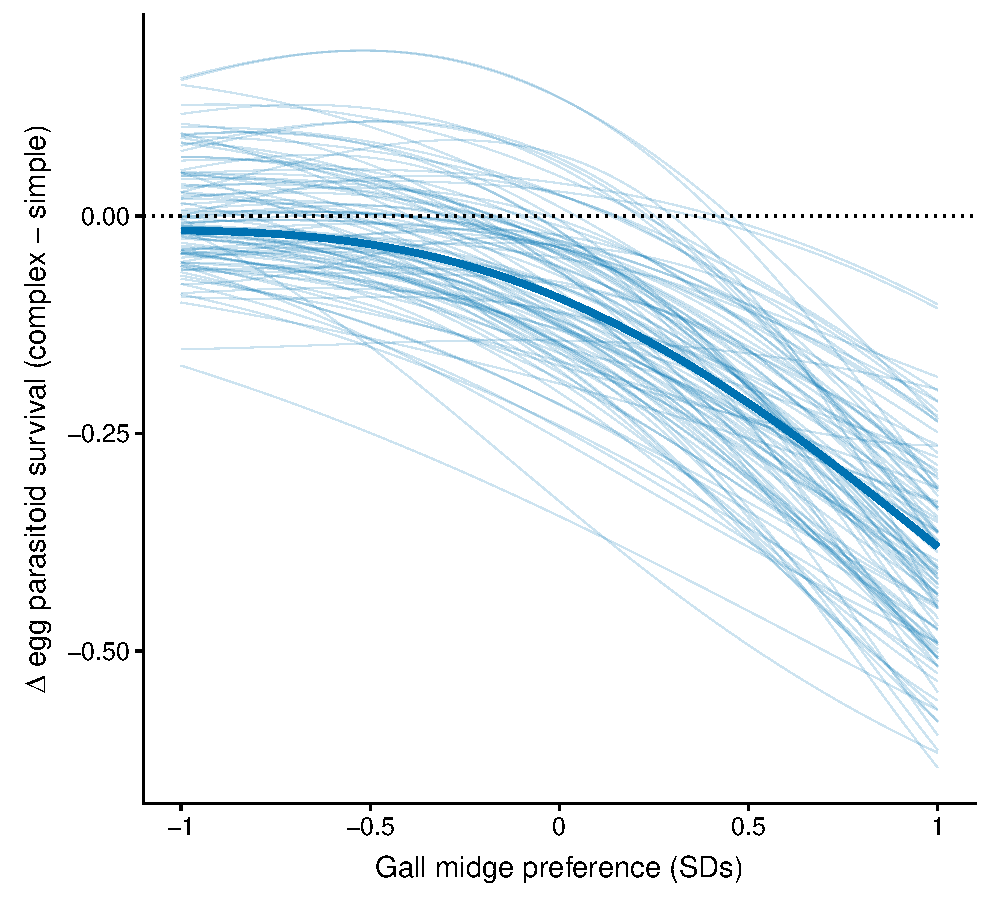
\includegraphics{analyses/selection_on_Platygaster.pdf}
\caption{\label{fig:EggPtoid_Selection}Selection imposed by larval
parasitoids on the extended phenotype of egg parasitoids
(\emph{Platygaster} sp.). The solid line represents the average
difference in the probability of observing the egg parasitoid in complex
vs.~simple food webs as a function of gall midge oviposition preference.
Transparent lines represent bootstrapped replicates to show the
uncertainty in selection. For clarity, we only display 100 bootstraps
even though inferences are based on 1,000 replicates. The decrease in
the probability of observing egg parasitoids at high gall-midge
densities indicate that larval parasitoids impose nonlinear selection on
the extended phenotype of egg parasitoids.}
\end{figure}

\bibliography{references}

\end{document}
